\documentclass[12pt]{article}  
% Эта строка — комментарий, она не будет показана в выходном файле  
\usepackage{ucs} 
\usepackage[utf8x]{inputenc} % Включаем поддержку UTF8  
\usepackage[russian]{babel}  % Включаем пакет для поддержки русского языка  
\usepackage{amsmath}
\usepackage{listings}
\usepackage{color}
\usepackage{tikz}
\usepackage{pgfplots}
\usepackage{filecontents}
\usepackage{graphicx}


\definecolor{mygreen}{rgb}{0,0.6,0}
\definecolor{mygray}{rgb}{0.5,0.5,0.5}
\definecolor{mymauve}{rgb}{0.58,0,0.82}
\title{Отчет по лабораторной работе 1 \\ 
	По предмету “Анализ алгоритмов” \\
	По теме “Умножение матриц”
}  
\date{2018}  
\author{Фирсова Дарья ИУ7-56}

\begin{document}  
	\maketitle  
	\newpage
	\section*{Введение}
	В лабораторной работе изучаются алгоритмы умножения матриц. Использован стандартный, алгоритм Винограда и улучшенный алгоритм Винограда. Задачи для лабораторной работы:
\begin{enumerate}
	\item Ввести модель подсчета трудоемкости
	\item Реализовать стандартный алгоритм умножения матриц
	\item Реализовать алгоритм Винограда
	\item Релизовать улучшенный алгоритм Винограда, при этом произвести не менее 3 улучшений).
	\item Провести временные замеры
	\item Произвести рассчет трудоемкости для реализованных алгоритмов.
\end{enumerate}
\newpage

\section{Аналитеская часть}
В данном разделе приведены алгоритмы и составлена модель для вычисления трудоемкости.
\subsection{Описание алгоритмов}

\subsubsection{Стандартный алгоритм умножения. }

Имеем две матрицы A и B размерностями M x N и N x Q соответственно. \\Тогда результирующей матрицей будет матрица С размером M x Q, где $c_{ij}$ = $\sum_{r=1}^n a_{ir}\cdot b_{rj} ,   (i = 0,1,2...m, j = 0,1,2...q)$.
\\
\\
\subsubsection{Алгоритм Винограда.}
Пусть $i$-я строка матрицы A - вектор  $\vec{U}$, а $j$-й столбец матрицы B - вектор $\vec{V}$. \\
Тогда $C_{ij}$ = \begin{tabular}{|c|c|c|c|}
	\hline
	$u_{1}$  $u_{2}$  $u_{3}$  $u_{4}$ \\
	\hline
\end{tabular} $\cdot$ 
\begin{tabular}{|c|}
	\hline
	$v_{1}$ \\
	$v_{2}$  \\
	$v_{3}$   \\
	$v_{4}$  \\
	\hline
\end{tabular}
= $u_{1}$$v_{1}$ + $u_{2}$$v_{2}$ + $u_{3}$$v_{3}$ + $u_{4}$$v_{4}$ = \\
($u_{1}$+$v_{2}$)($u_{2}$$v_{1}$) + ($u_{3}$+$v_{4}$)($u_{4}$+$v_{3}$) - $u_{1}$$u_{2}$ - $u_{3}$$u_{4}$ - $v_{1}$$v_{2}$ - $v_{3}$$v_{4}$. \\

Хвост для  $\vec{U}$ вычисляется заранее и используется повтороно при умножении на каждый столбец матрицы B.

Если вектора $\vec{U}$ и $\vec{V}$ нечетной длины, то к приведенным выше вычислениям, добавляем 
$C_{ij}$ += $U_{N-1}\cdot V_{N-1}, \forall i,j$
\\

\subsection{Модель вычислений}
Введем следующую модель вычислений:
операции $+$  $-$  $*$  $/$  $<$  $>$  $==$  $!=$  $+=$  $=$  $[]$  имеют стоимость 1.
\\
\\
\subsubsection{Оценка трудоемкости цикла for}
Инициализация до цикла стоит 2, после выполнения тела цикла, инкрементируется итератор цикла, проверяется условие.
\\
$F = 2 + N*(F_{body} + 2)$

\subsubsection{Оценка трудоемкости оператора if}
Переход по условию имеет стоимость 0, проверка условия зависит от выражения самой провеки
\\
{$F_{if1} =0$\\$F_{if2} = 0 + body$}
\subsubsection{Оценка трудоемкости стандартного алгоритма}
$13MNQ+4MQ+4M+2$
\subsubsection{Оценка трудоемкости алгоритма Винограда}
Первая часть: $\dfrac{13MN}{2}+5M+2$ \\
Вторая часть: $\dfrac{13QN}{2}+5M+2$ \\
Третья часть $12MNQ+9MQ+2M+2$ \\
Четвертая часть: $15QM+2M+1$ \\

\subsubsection{Оценка трудоемкости улучшенного алгоритма Винограда}
Первая часть: $6MN+2M+2$ \\
Вторая часть: $6QN+2M+2$ \\
Третья часть $10MNQ+9QM+2M+2$ \\
Четвертая часть: $12MQ + 2M + 1$ \\
\newpage
\section{Конструкторская часть}
В данном разделе представлены схемы алгоритмов 

\begin{figure}[ht!]
	\centering
	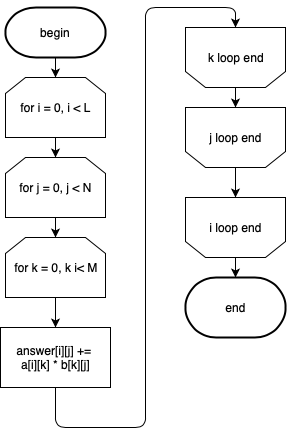
\includegraphics[width=30mm, height=180mm]{multiply.png}
	\caption{Схема стандартного алгоритма\label{overflow}}
\end{figure}
\begin{figure}[ht!]
	\centering
	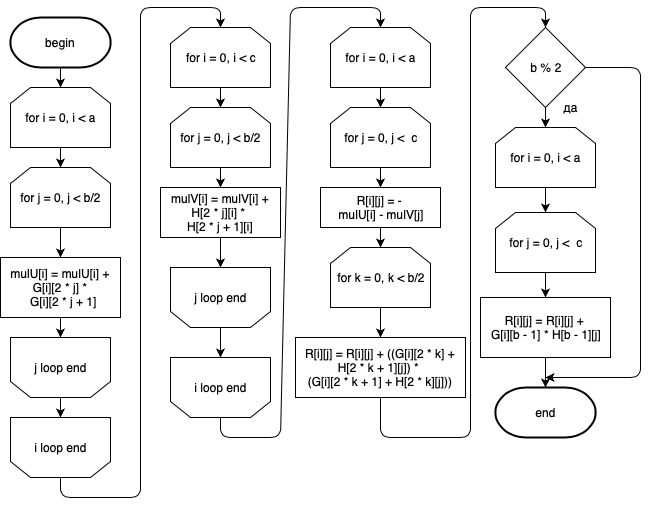
\includegraphics[width=130mm, height=150mm]{wino.png}
	\caption{Схема алгоритма Винограда \label{overflow}}
\end{figure}

\newpage

\newpage
\section{Технологическая часть}

В этом разделе приведена реализация функций, указан язык программирования и необходимые модули. 
\subsection{Требования к программному обеспечению}

\subsection{Средства реализации}
В данной работе использовался язык Python 3.6, в среде Pycharm. Для измерения времени использовался модуль time.
\subsection{Листинг кода}
\lstset{ 
	backgroundcolor=\color{white},   % choose the background color; you must add \usepackage{color} or \usepackage{xcolor}; should come as last argument
	basicstyle=\footnotesize,        % the size of the fonts that are used for the code
	breakatwhitespace=false,         % sets if automatic breaks should only happen at whitespace
	breaklines=true,                 % sets automatic line breaking
	captionpos=b,                    % sets the caption-position to bottom
	commentstyle=\color{mygreen},    % comment style
	deletekeywords={...},            % if you want to delete keywords from the given language
	escapeinside={\%*}{*)},          % if you want to add LaTeX within your code
	extendedchars=true,              % lets you use non-ASCII characters; for 8-bits encodings only, does not work with UTF-8
	frame=single,	                   % adds a frame around the code
	keepspaces=true,                 % keeps spaces in text, useful for keeping indentation of code (possibly needs columns=flexible)
	keywordstyle=\color{blue},       % keyword style
	language=Python,                 % the language of the code
	morekeywords={*,...},            % if you want to add more keywords to the set
	numbers=left,                    % where to put the line-numbers; possible values are (none, left, right)
	numbersep=5pt,                   % how far the line-numbers are from the code
	numberstyle=\tiny\color{mygray}, % the style that is used for the line-numbers
	rulecolor=\color{black},         % if not set, the frame-color may be changed on line-breaks within not-black text (e.g. comments (green here))
	showspaces=false,                % show spaces everywhere adding particular underscores; it overrides 'showstringspaces'
	showstringspaces=false,          % underline spaces within strings only
	showtabs=false,                  % show tabs within strings adding particular underscores
	stepnumber=1,                    % the step between two line-numbers. If it's 1, each line will be numbered
	stringstyle=\color{mymauve},     % string literal style
	tabsize=2,	                   % sets default tabsize to 2 spaces
	title=\lstname                   % show the filename of files included with \lstinputlisting; also try caption instead of title
}
\lstinputlisting[language=Python]{functions.py}
\newpage

\newpage
\newpage

\section{Экспериментальная часть}
В данном разделе будут приведены примеры работы алгоритмов и приведены замеры времени. Тестирование производилось на компьютере с процессором Intel Core i5 (I5-6267U) и оперативной памятью 8 Гб. 
\subsection{Примеры работы}

	Пример результата работы умножения матриц. Так как в данной реализации генерируются случайные значения, то для проверки результата использовалась библиотека Numpy. 
	\newline

$$\begin{bmatrix} 
12 & 14 & 20 \\
24 & 14 & 16 \\
\end{bmatrix}$$
+
$$\begin{bmatrix} 
11 &15\\
8 & 15 \\
14 & 15 \\
\end{bmatrix}$$
=
$$\begin{bmatrix} 
524 & 690 \\
600 & 810 \\
\end{bmatrix}$$

\subsection{Сравнительный анализ}
Сравнение алгоритмов стандартного умножения, алгоритма Винограда и улучшенного алгоритма Винограда.
\newline
\begin{tikzpicture}
\begin{axis}
[
axis x line=middle,
axis y line=middle,
enlarge y limits=true,
xmin=0, xmax=200,
ymin=0, ymax=5000,
width=15cm, height=15cm,     % size of the image
grid = major,
grid style={dashed, gray!30},
ylabel=Время,
xlabel=Длина,
legend style={at={(0.1,-0.1)}, anchor=north}
]
\addplot table [x=length, y=basic, col sep=comma] {out.txt};
\addplot table [x=length, y=wino, col sep=comma] {out.txt};
\addplot table [x=length, y=opt, col sep=comma] {out.txt};
\legend {Обычный, Виноград, Улучшеный}
\end{axis}
\end{tikzpicture}

\subsection{Заключение}
На больших значениях данных улучшенный алгоритм Винограда 
\section{Вывод}
В данной лабораторной работе вычислены сложности алгоритмов для умножения матриц. Разработаны программы по этим алгоритмам, проведены тесты по времени, произведен сравнительный анализ алгоритмов. Для составления отчета использован Latex.
\\
\end{document}